% \documentclass[aspectratio=169,notes]{beamer}
\documentclass[aspectratio=169]{beamer}
\usetheme[faculty=phil]{fibeamer}
\usepackage{polyglossia}
\setmainlanguage{english} %% main locale instead of `english`, you
%% can typeset the presentation in either Czech or Slovak,
%% respectively.
\setotherlanguages{russian} %% The additional keys allow
%%
%%   \begin{otherlanguage}{czech}   ... \end{otherlanguage}
%%   \begin{otherlanguage}{slovak}  ... \end{otherlanguage}
%%
%% These macros specify information about the presentation
\title[MaM]{Mechanics and Machines, Lecture 3} %% that will be typeset on the
\subtitle{Types of drives: kinematics, where to find other info
\\ Drives: friction, belts, chains, gears, universal, geneva       \\ \  
         } %% title page.
\author{Oleg Bulichev}
%% These additional packages are used within the document:
\usepackage{ragged2e}  % `\justifying` text
\usepackage{booktabs}  % Tables
\usepackage{tabularx}
\usepackage{tikz}      % Diagrams
\usetikzlibrary{calc, shapes, backgrounds}
\usepackage{amsmath, amssymb}
\usepackage{url}       % `\url`s
\usepackage{listings}  % Code listings
% \usepackage{subfigure}
\usepackage{floatrow}
\usepackage{subcaption}
\usepackage{mathtools}
\usepackage{todonotes}
\usepackage{fontspec}
\usepackage{multicol}
\usepackage{pdfpages}
\usepackage{wrapfig}
\usepackage{animate}
\usepackage{booktabs}
\usepackage{multirow}
% \usepackage{graphicx}
\usepackage{colortbl}

\graphicspath{{resources/}}
\frenchspacing

\setbeamertemplate{caption}[numbered]
\usetikzlibrary{graphs}

% \usepackage[backend=biber,style=ieee,autocite=footnote]{biblatex}
% \addbibresource{biblio.bib}
% \DefineBibliographyStrings{english}{%
%   bibliography = {References},}

\newcommand{\oleg}[2][] {\todo[color=red, #1] {OLEG:\\ #2}}
\newcommand{\fbckg}[1]{\usebackgroundtemplate{\includegraphics[width=\paperwidth]{#1}}}%frame background

\usepackage[framemethod=TikZ]{mdframed}
\newcommand{\dbox}[1]{
\begin{mdframed}[roundcorner=3pt, backgroundcolor=yellow, linewidth=0]
\vspace{1mm}
{#1}
\vspace{1mm}
\end{mdframed}
}

\begin{document}
\setlength{\abovedisplayskip}{0pt}
\setlength{\belowdisplayskip}{0pt}
\setlength{\abovedisplayshortskip}{0pt}
\setlength{\belowdisplayshortskip}{0pt}

\fbckg{fibeamer/figs/title_page.png}
\frame[c]{\setcounter{framenumber}{0}
    \usebeamerfont{title}%
    \usebeamercolor[fg]{title}%
    \begin{minipage}[b][6.5\baselineskip][b]{\textwidth}%
        \textcolor{black}{\raggedright\inserttitle}
    \end{minipage}
    % \vskip-1.5\baselineskip

    \usebeamerfont{subtitle}%
    \usebeamercolor[fg]{framesubtitle}%
    \begin{minipage}[b][3\baselineskip][b]{\textwidth}
        \raggedright%
        \insertsubtitle%
    \end{minipage}
    \vskip.25\baselineskip
}
%   \frame[c]{\maketitle}

\fbckg{fibeamer/figs/common.png}

\note{\scriptsize \begin{itemize}
        \item \
    \end{itemize}}

\begin{frame}[c]{Goal of the lecture}
    \framesubtitle{}
    \LARGE
    \centering
    Make an overview of typical drives. \\ Give a hint how to work with it. \\ Explain how to find information about particular drive.
\end{frame}

\begin{frame}[t]{Universal Joint}
    \framesubtitle{Visualisation}
    \vspace{-0.5cm}
    \begin{figure}[H]
        \begin{subfigure}{0.49\textwidth}
            \centering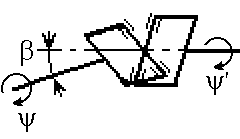
\includegraphics[height=6cm,width=1\textwidth,keepaspectratio]{universal_kinematics.png}
        \end{subfigure}
        \begin{subfigure}{0.49\textwidth}
            \href{https://en.wikipedia.org/wiki/Universal_joint\#/media/File:Universal_joint.gif}{
                \centering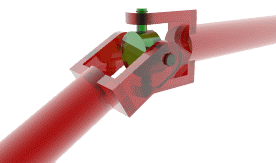
\includegraphics[height=6cm,width=1\textwidth,keepaspectratio]{cardan_video_preview.png}}
        \end{subfigure}
    \end{figure}
\end{frame}


\begin{frame}[t]{Universal Joint}
    \framesubtitle{Types of universal joint}
    \begin{figure}[H]
        \begin{subfigure}{0.32\textwidth}
            \centering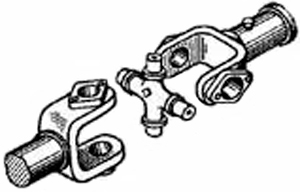
\includegraphics[height=6cm,width=1\textwidth,keepaspectratio]{universal_1.png}
            \caption*{Cardan}
        \end{subfigure}
        \begin{subfigure}{0.32\textwidth}
            \href{https://en.wikipedia.org/wiki/Constant-velocity_joint\#/media/File:Double_Cardan_Joint_(animated).gif}{
                \centering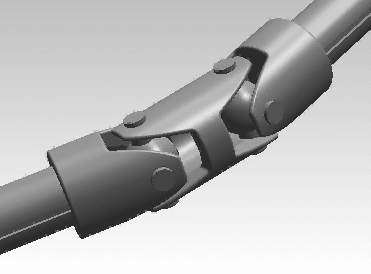
\includegraphics[height=6cm,width=1\textwidth,keepaspectratio]{universal_2_video_preview.png}}
            \caption*{Double cardan joint}
        \end{subfigure}
        \begin{subfigure}{0.32\textwidth}
            \href{https://gifyu.com/image/SqMnR}{
                \centering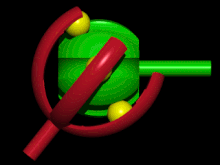
\includegraphics[height=6cm,width=1\textwidth,keepaspectratio]{shrus_video_preview.png}}
            \caption*{Constant-velocity universal ball joint}
        \end{subfigure}
    \end{figure}
\end{frame}

\begin{frame}[t]{Universal Joint}
    \framesubtitle{Drive kinematics (1)}
    \begin{columns}[T,onlytextwidth]
        \begin{column}{0.59\textwidth}
            Angle relationship --- $\tan(\psi)=\tan(\psi')\cos(\beta)$ \\
            Angular velocities relationship --- $ \omega \cos(\beta) = \omega'(\sin^2(\psi) + \cos^2(\psi)\cos^2(\beta))$
        \end{column}
        \begin{column}{0.39\textwidth}
            \vspace{-0.9cm}
            \begin{figure}[H]
                \centering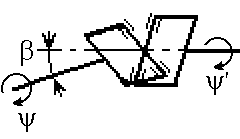
\includegraphics[height=6cm,width=1\textwidth,keepaspectratio]{universal_kinematics.png}
                % \caption{caption_name}
                \label{fig:universal_kinematics.png}
            \end{figure}
        \end{column}
    \end{columns}

\end{frame}

\begin{frame}[t]{Universal Joint}
    \framesubtitle{Features and facts}
    \begin{itemize}
        \item It's effective tool for transferring a torque for max 30 degrees.
        \item Constant-velocity universal ball joint (шрус) is not a small device and it's not easy to find it (it can be found as a car detail).
    \end{itemize}
\end{frame}

\begin{frame}[t]{Universal Joint}
    \framesubtitle{What can be interesting to find (queries)}
    \begin{enumerate}
        \item Correlation between velocities and angle between links in Universal joint
        \item Cardan dynamics
    \end{enumerate}
\end{frame}

\begin{frame}[t]{Universal Joint}
    \framesubtitle{Reference material}
    \begin{enumerate}
        \item \textbf{Other names}: cardan joint, Hooke's joint, кардан, универсальный шарнир
        \item \href{https://en.wikipedia.org/wiki/Universal_joint}{Universal joint (wiki)}
        \item \textit{"Теория механизмов и машин" Артоболевский И. И. 1988, pdf pages 168--172 }
        \item \href{https://elar.urfu.ru/bitstream/10995/102516/1/2-s2.0-85107367228.pdf}{Find U-joint parameters using quaternions}
        \item \href{https://www.researchgate.net/publication/257774799_Dynamics_of_universal_joints_its_failures_and_some_propositions_for_practically_improving_its_performance_and_life_expectancy}{Dynamics of universal joints}
    \end{enumerate}
\end{frame}

\begin{frame}[t]{Belt}
    \framesubtitle{Visualisation}
    \vspace{-0.5cm}
    \begin{figure}[H]
        \begin{subfigure}{0.49\textwidth}
            \centering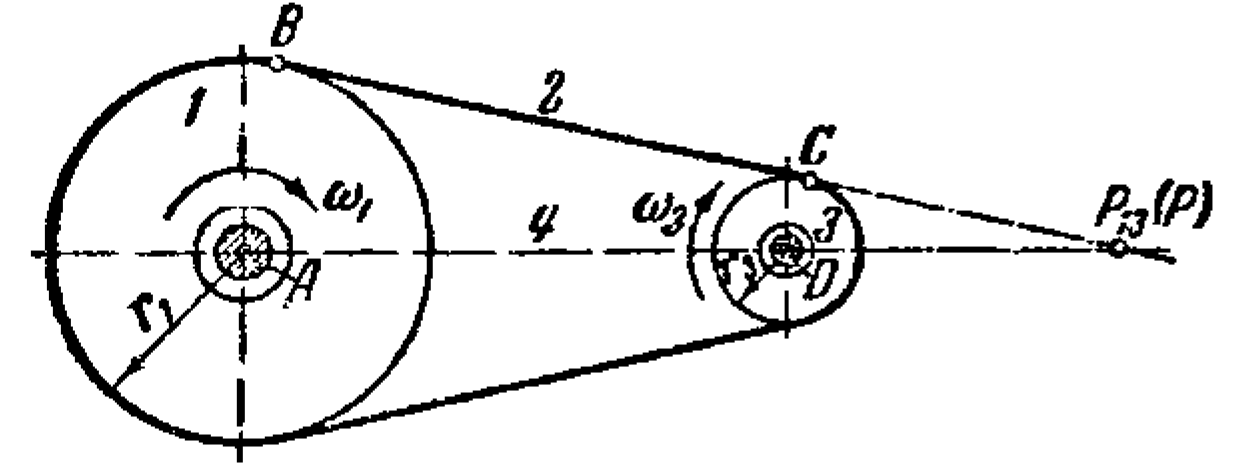
\includegraphics[height=2.6cm,width=1\textwidth,keepaspectratio]{belt_kinematics_1.png}
            % \caption{capture1}
            \label{fig:belt_kinematics_1.png}
        \end{subfigure}
        \begin{subfigure}{0.49\textwidth}
            \centering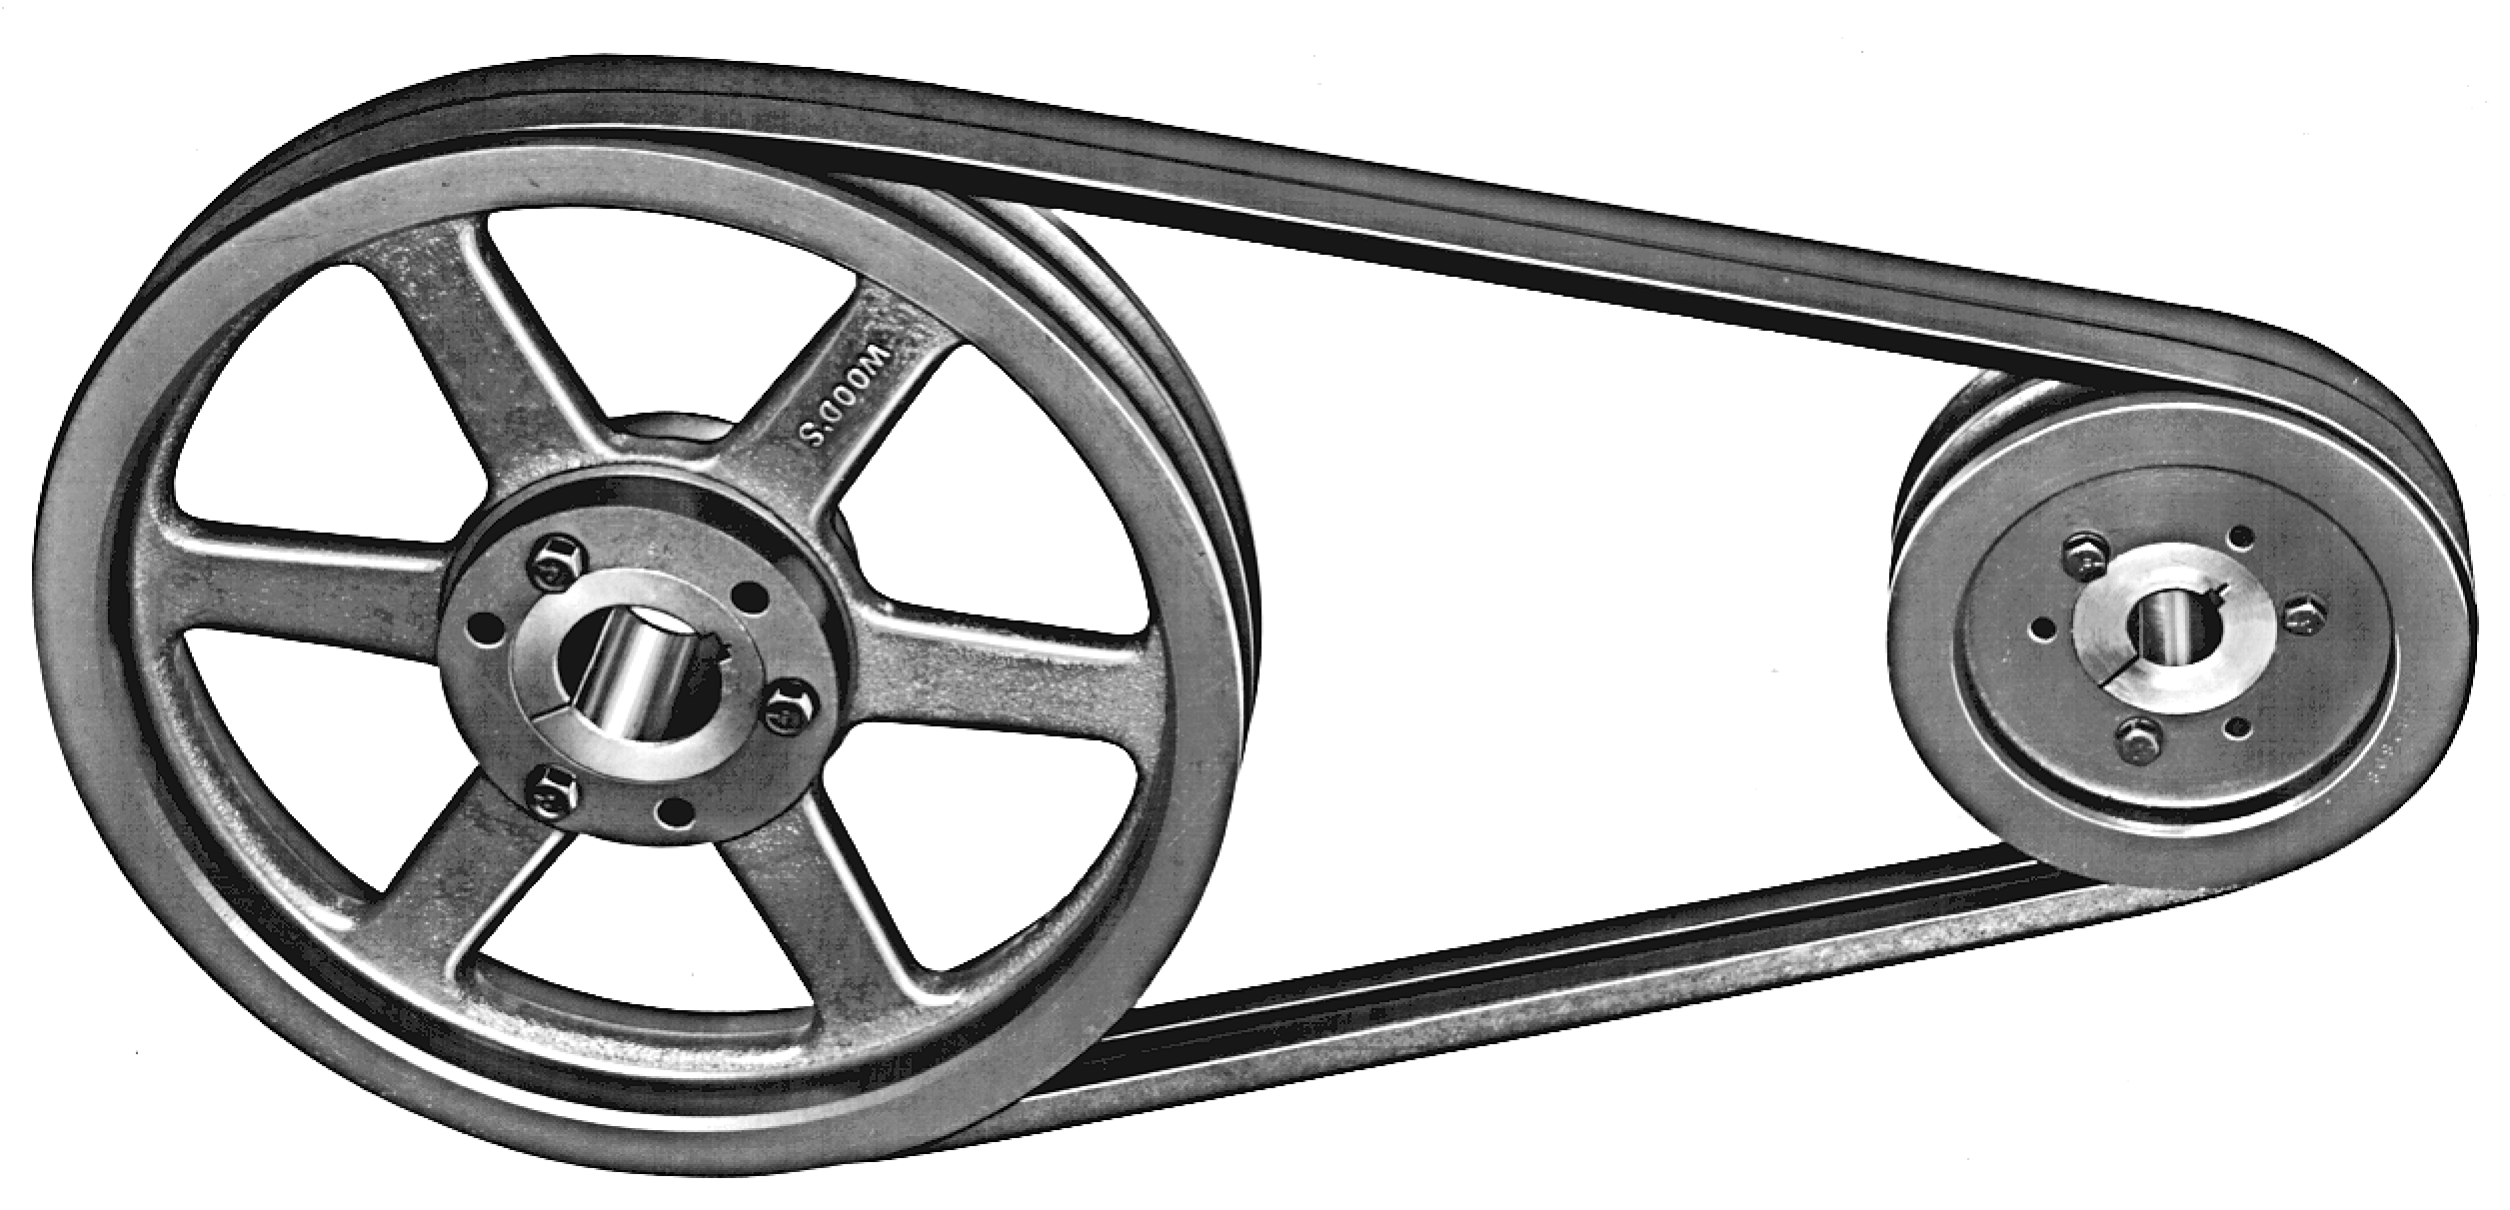
\includegraphics[height=2.6cm,width=1\textwidth,keepaspectratio]{belt_1.png}
            % \caption{capture2}
            \label{fig:belt_1.png}
        \end{subfigure}

        \begin{subfigure}{0.49\textwidth}
            \centering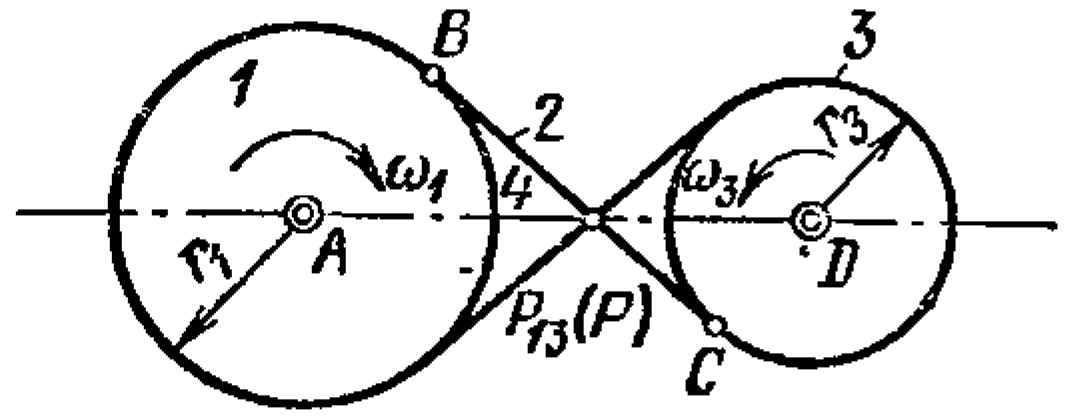
\includegraphics[height=2.6cm,width=1\textwidth,keepaspectratio]{belt_kinematics_2.png}
            % \caption{capture1}
            \label{fig:belt_kinematics_2.png}
        \end{subfigure}
        \begin{subfigure}{0.49\textwidth}
            \centering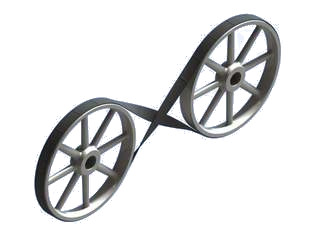
\includegraphics[height=3.1cm,width=1\textwidth,keepaspectratio]{belt_2.jpg}
            % \caption{capture2}
            \label{fig:belt_2.jpg}
        \end{subfigure}
    \end{figure}
\end{frame}

\begin{frame}[t]{Belt}
    \framesubtitle{Types of belts}
    \vspace{-1.2cm}
    \begin{figure}[H]
        \centering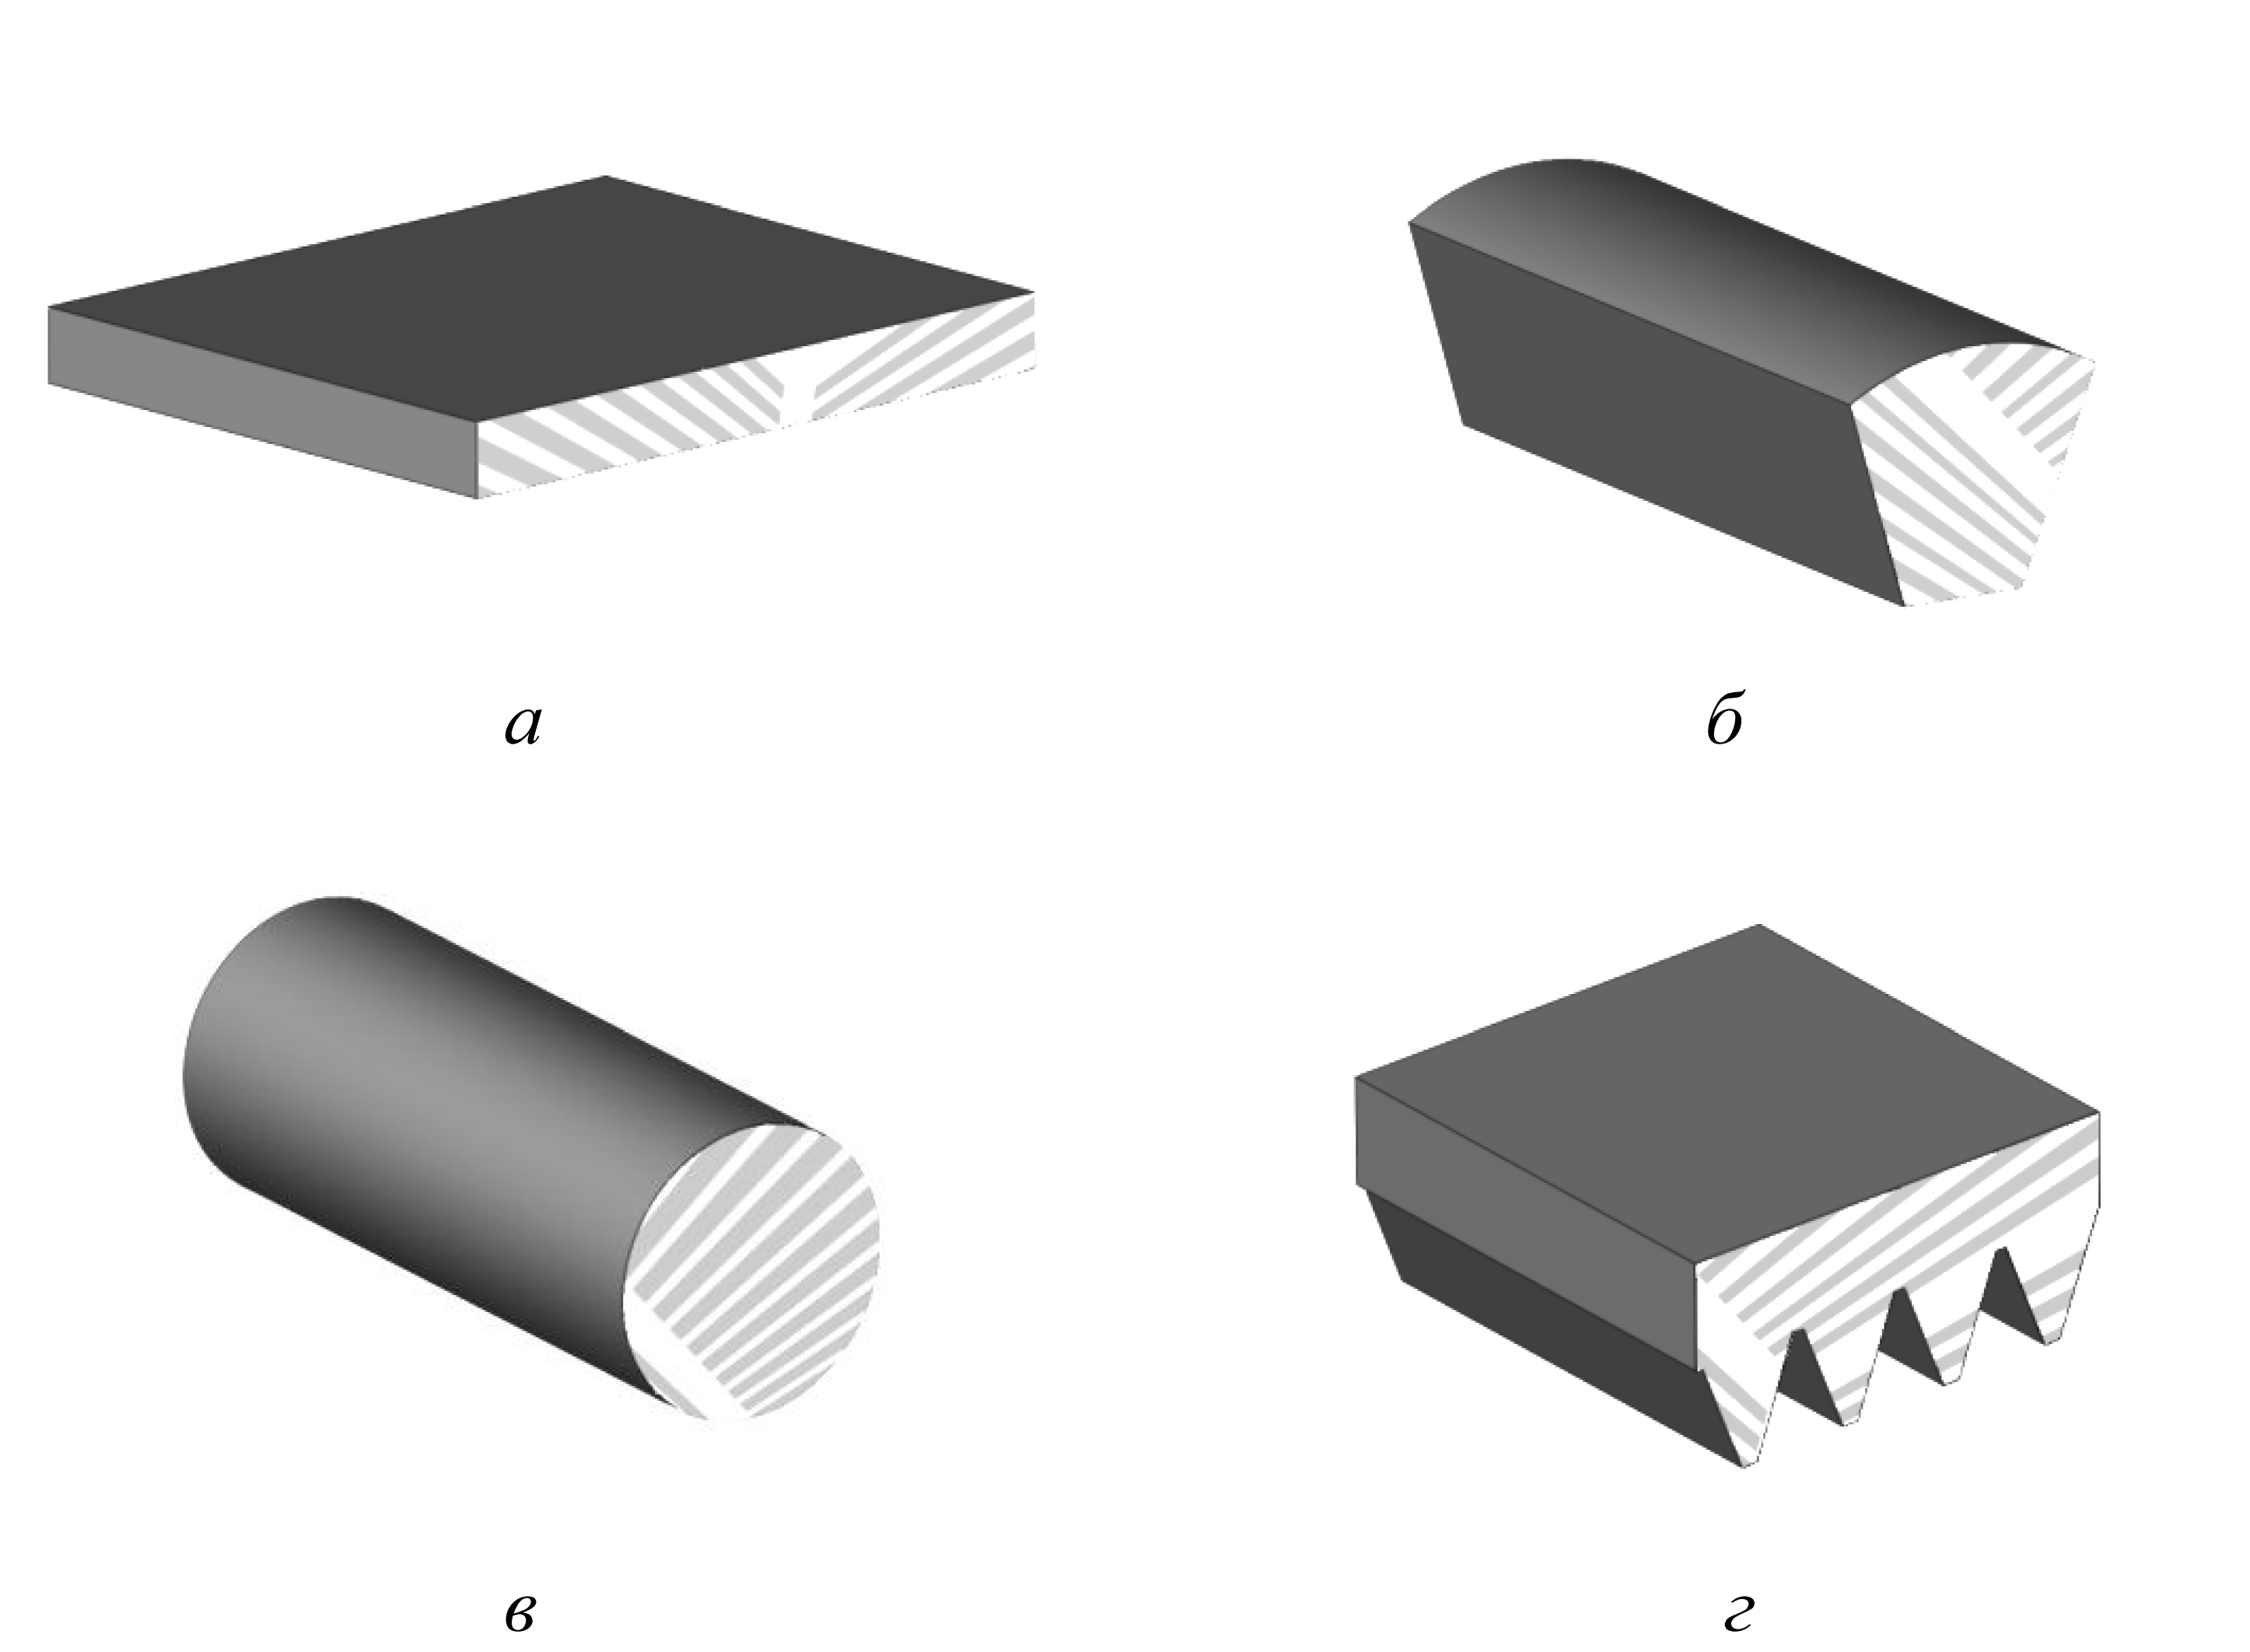
\includegraphics[height=6cm,width=1\textwidth,keepaspectratio]{belt_types.png}
        \caption*{\textit{а}) flat (плоская), \textit{б}) vee belt (клиновидная), \textit{в}) round (круглая), \textit{г}) timing (toothed, зубчатый)}
        \label{fig:belt_types.png}
    \end{figure}

\end{frame}

\begin{frame}[t]{Belt}
    \framesubtitle{Drive kinematics (1)}
    \begin{itemize}
        \item Linear velocity of a pulley --- $v_1=\omega_1 \frac{d_1}{2}$, $d$ --- diameter of a pulley (шкив)
        \item Length of pulley --- $l = 2a + \frac{\pi}{2}(d_1 + d_2) + \dfrac{(d_2-d_1)^2}{4a}$, where $a$ --- distance between center of pulleys.
    \end{itemize}
\end{frame}


\begin{frame}[t]{Belt}
    \framesubtitle{What can be interesting to find (queries)}
    \begin{itemize}
        \item How to find the appropriate diameter of a pulley
        \item Min and max distance between pulleys
        \item Appropriate angle of covering the pulley
    \end{itemize}
\end{frame}

\begin{frame}[t]{Belt}
    \framesubtitle{Features and facts}
    \begin{itemize}
        \item Simple design and operation, relatively low cost. 
        \item Smooth and quiet operation due to elasticity belt. 
        \item Possibility to transfer power over long distances (with V-belts up to 15 m) at speed up to 100 m/s. 
        \item Softening of vibrations and shocks due to elasticity of the belt. 
        \item Possibility to protect machines from overloading due to elastic belt tension and slippage  
        \item Reduced requirements for axle alignment 
        shafts.
    \end{itemize}
\end{frame}

\begin{frame}[t]{Belt}
    \framesubtitle{Reference material}
    \begin{enumerate}
        \item \textbf{Other names}: ременная передача
        \item \href{https://en.m.wikipedia.org/wiki/Belt_(mechanical)}{Belt drive (wiki)}
        \item \textit{"Теория механизмов и машин" Артоболевский И. И. 1988, pdf pages 166--168 }
        \item \href{https://studfile.net/preview/2156455/}{Детали машин. 9 лекция}
        \item \href{https://youtu.be/CP_b7bzM9nQ}{Belt formulas}
    \end{enumerate}
\end{frame}


\begin{frame}[t]{Chain}
    \framesubtitle{Visualisation}
    \vspace{-1cm}
    \begin{figure}[H]
        \begin{subfigure}[c]{0.49\textwidth}
            \centering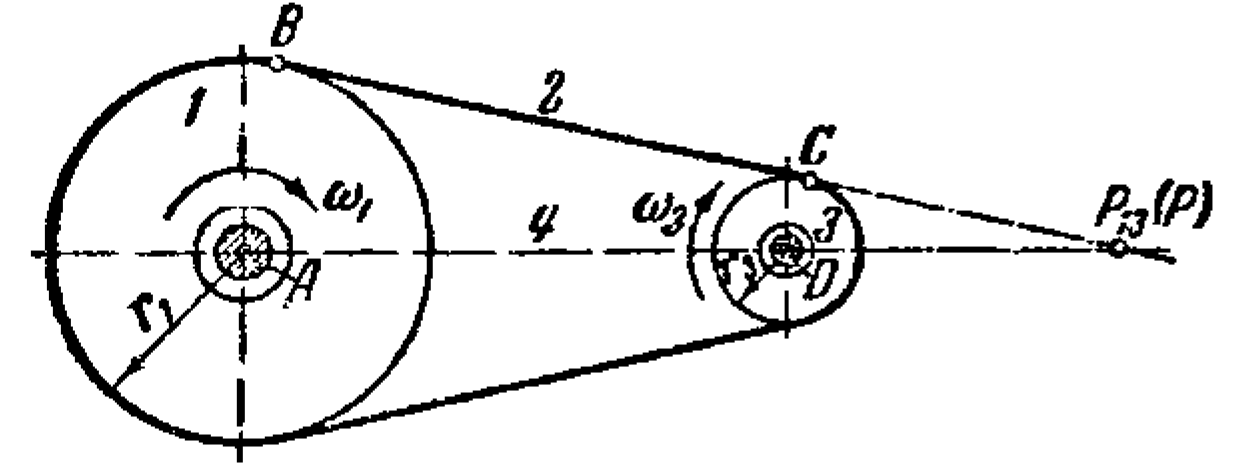
\includegraphics[height=6cm,width=1\textwidth,keepaspectratio]{belt_kinematics_1.png}
        \end{subfigure}
        \begin{subfigure}[c]{0.49\textwidth}
            \centering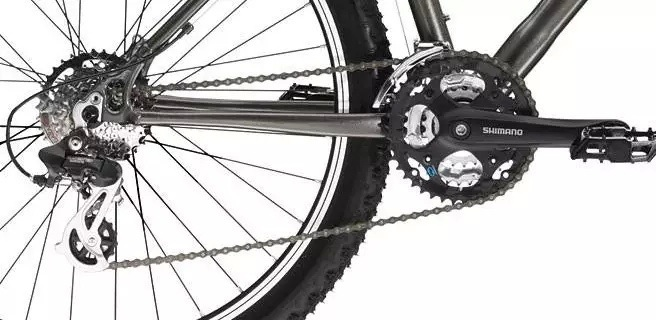
\includegraphics[height=6cm,width=1\textwidth,keepaspectratio]{chain_1.jpg}
            % \caption{capture2}
            \label{fig:chain_1.jpg}
        \end{subfigure}

        \begin{subfigure}[c]{0.5\textwidth}
            \centering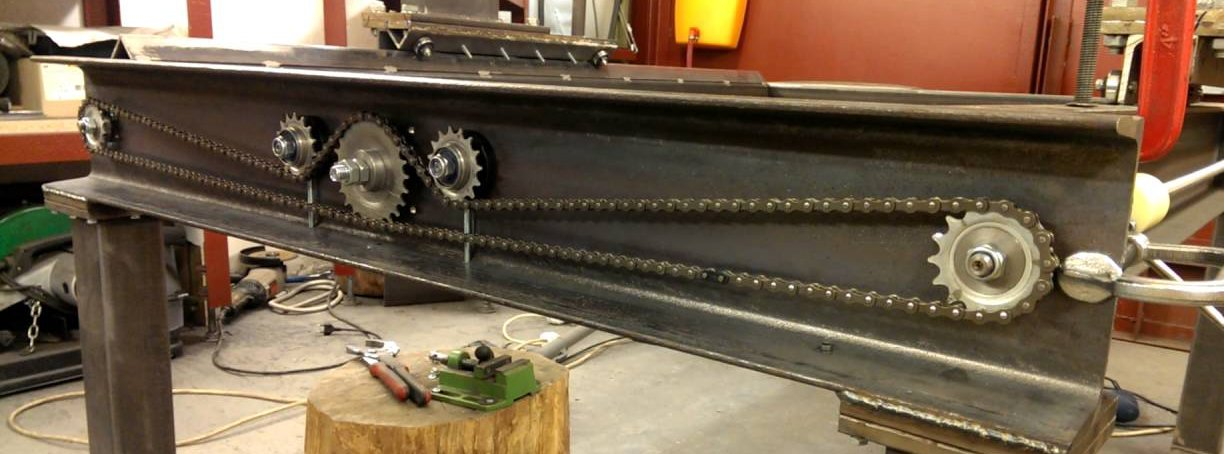
\includegraphics[height=6cm,width=1\textwidth,keepaspectratio]{chain_2.jpg}
            % \caption{capture2}
            \label{fig:chain_2.jpg}
        \end{subfigure}
    \end{figure}
\end{frame}

\begin{frame}[t]{Chain}
    \framesubtitle{Types of chain transmissions}

\end{frame}

\begin{frame}[t]{Chain}
    \framesubtitle{Drive kinematics (1)}

\end{frame}

\begin{frame}[t]{Chain}
    \framesubtitle{Drive kinematics (2)}

\end{frame}

\begin{frame}[t]{Chain}
    \framesubtitle{What can be interesting to find (queries)}

\end{frame}

\begin{frame}[t]{Chain}
    \framesubtitle{Reference material}
    \begin{enumerate}
        \item \textbf{Other names}: цепная передача
        \item \href{https://en.wikipedia.org/wiki/Roller_chain}{Roller chain (wiki)}
        \item \textit{"Теория механизмов и машин" Артоболевский И. И. 1988, pdf pages 166--168 }
        \item \href{https://studfile.net/preview/2156460/}{Детали машин. 10 лекция}
        \item \href{https://www.youtube.com/watch?v=F7o3LOtKEA8}{Sprockets \& Chains For Engineers}
    \end{enumerate}
\end{frame}

\begin{frame}[t]{Geneva drive}
    \framesubtitle{Visualisation}
    \vspace{-0.5cm}
    \begin{figure}[H]
        \begin{subfigure}{0.49\textwidth}
            \centering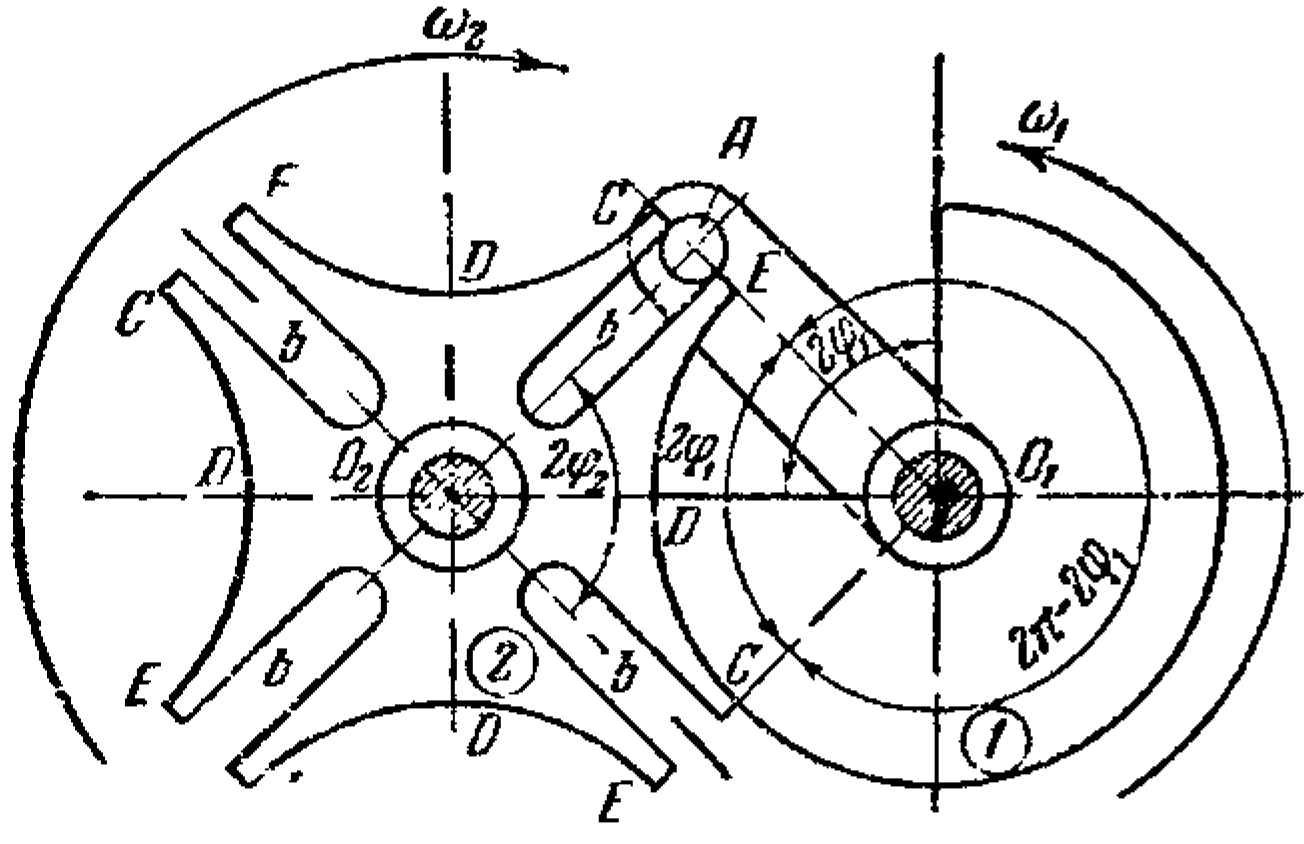
\includegraphics[height=6cm,width=1\textwidth,keepaspectratio]{geneva_kinematics.png}
        \end{subfigure}
        \begin{subfigure}{0.49\textwidth}
            \href{https://en.wikipedia.org/wiki/Geneva_drive\#/media/File:Geneva_mechanism_6spoke_animation.gif}{
                \centering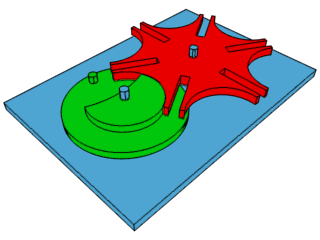
\includegraphics[height=6cm,width=1\textwidth,keepaspectratio]{Geneva_drive_video_preview.png}}
        \end{subfigure}
    \end{figure}    
\end{frame}

\begin{frame}[t]{Geneva drive}
    \framesubtitle{Types of geneva drive}

\end{frame}

\begin{frame}[t]{Geneva drive}
    \framesubtitle{Drive kinematics (1)}

\end{frame}

\begin{frame}[t]{Geneva drive}
    \framesubtitle{Drive kinematics (2)}

\end{frame}

\begin{frame}[t]{Geneva drive}
    \framesubtitle{What can be interesting to find (queries)}

\end{frame}

\begin{frame}[t]{Geneva drive}
    \framesubtitle{Reference material}
    \begin{enumerate}
        \item \textbf{Other names}: мальтийский крест
        \item \href{https://en.wikipedia.org/wiki/Geneva_drive}{Geneva drive (wiki)}
        \item \textit{"Теория механизмов и машин" Артоболевский И. И. 1988, pdf pages 172--174 }
        \item \href{https://www.youtube.com/watch?v=1lyWywC_z4o}{How to draw a geneva drive}
    \end{enumerate}
\end{frame}

\begin{frame}[t]{Friction drive}
    \framesubtitle{Visualisation}

\end{frame}

\begin{frame}[t]{Friction drive}
    \framesubtitle{Types of friction drive}

\end{frame}

\begin{frame}[t]{Friction drive}
    \framesubtitle{Drive kinematics (1)}

\end{frame}

\begin{frame}[t]{Friction drive}
    \framesubtitle{Drive kinematics (2)}

\end{frame}

\begin{frame}[t]{Friction drive}
    \framesubtitle{What can be interesting to find (queries)}

\end{frame}

\begin{frame}[t]{Friction drive}
    \framesubtitle{Reference material}
    \begin{enumerate}
        \item \textbf{Other names}: фрикционная передача
        \item \href{https://en.m.wikipedia.org/wiki/Friction_drive}{Friction drive (wiki)}
        \item \textit{"Теория механизмов и машин" Артоболевский И. И. 1988, pdf pages 141--146 }
        \item \href{https://studfile.net/preview/2156467/page:2/}{Детали машин. 22 лекция, 2 страница}
        \item 
    \end{enumerate}
\end{frame}

\begin{frame}[t]{Gears}
    \framesubtitle{Visualisation}

\end{frame}

\begin{frame}[t]{Gears}
    \framesubtitle{Types of Gears}

\end{frame}

\begin{frame}[t]{Gears}
    \framesubtitle{Drive kinematics (1)}

\end{frame}

\begin{frame}[t]{Gears}
    \framesubtitle{Drive kinematics (2)}

\end{frame}

\begin{frame}[t]{Gears}
    \framesubtitle{What can be interesting to find (queries)}

\end{frame}

\begin{frame}[t]{Gears}
    \framesubtitle{Reference material}
    \begin{enumerate}
        \item \textbf{Other names}: зубчатая передача
        \item \href{https://en.wikipedia.org/wiki/Gear}{Gears (wiki)}
        \item \textit{"Теория механизмов и машин" Артоболевский И. И. 1988, pdf pages 145--166 }
        \item \href{https://studfile.net/preview/2156468/}{Детали машин. 5-8 лекции}
        \item \textit{"Design of machinery" Robert L. Norton, pdf pages 517--557 } \textbf{2.0 --- 2.11}
    \end{enumerate}
\end{frame}

\begin{frame}[t]{Ballscrew}
    \framesubtitle{Visualisation}

\end{frame}

\begin{frame}[t]{Ballscrew}
    \framesubtitle{Types of ballscrew}

\end{frame}

\begin{frame}[t]{Ballscrew}
    \framesubtitle{Drive kinematics (1)}

\end{frame}

\begin{frame}[t]{Ballscrew}
    \framesubtitle{Drive kinematics (2)}

\end{frame}

\begin{frame}[t]{Ballscrew}
    \framesubtitle{What can be interesting to find (queries)}

\end{frame}

\begin{frame}[t]{Ballscrew}
    \framesubtitle{Reference material}
    \begin{enumerate}
        \item \textbf{Other names}: шарико-винтовая передача
        \item \href{https://en.wikipedia.org/wiki/Ball_screw}{Ball screw (wiki)}
        \item \textit{"Теория механизмов и машин" Артоболевский И. И. 1988, pdf pages 166--168 }
        \item \href{https://studfile.net/preview/2156460/}{Детали машин. 10 лекция}
        \item 
    \end{enumerate}
\end{frame}

\begin{frame}[t]{Reference material}
    % \Large
    \begin{itemize}
        \item \textit{"Mechanisms and Machines: Kinematics, Dynamics, and Synthesis" Michael M. Stanisic, pdf pages 21--56 } \textbf{1.1 --- 1.6}
        \item \textit{"Theory of Machines and Mechanisms" John J. Uicker, pdf pages 33--59 } \textbf{1.4 --- 1.7}
        \item \textit{"Design of machinery" Robert L. Norton, pdf pages 57--79 } \textbf{2.0 --- 2.11}
        \item \textit{"Механика. Теория механизмов и машин" Конищева О. В., pdf pages 7--23 } \\ Структурный анализ и классификация плоских механизмов
        \item \textit{"Теория механизмов и машин" Артоболевский И. И. 1988, pdf pages 21--63 } \\ Структурный анализ и классификация механизмов
              % \item \href{https://onlinemschool.com/math/library/vector/cos/}{Direction cosines (OnlineMSchool)}
    \end{itemize}
\end{frame}

\fbckg{fibeamer/figs/last_page.png}
\frame[plain]{}

\end{document}